\section*{Two Photon Decay}

The first step in the study of the branching ratio is the study of the Parapositroniu decay into two collinear photons. In order to converse linear momentum, the photons from the decay have to be emitted back to back with the same energy of 511 keV that is the p-Ps rest energy. In order to detect this kind of events, two detectors were placed at an angle of 180$^\circ$ as represented in Fig. \ref{Fig: exp setup for 2gamma}. Within this configuration, the spectra in Fig. \ref{Fig: 2gamma coinc with bg} are obtained.
\begin{figure}[H]
\centering
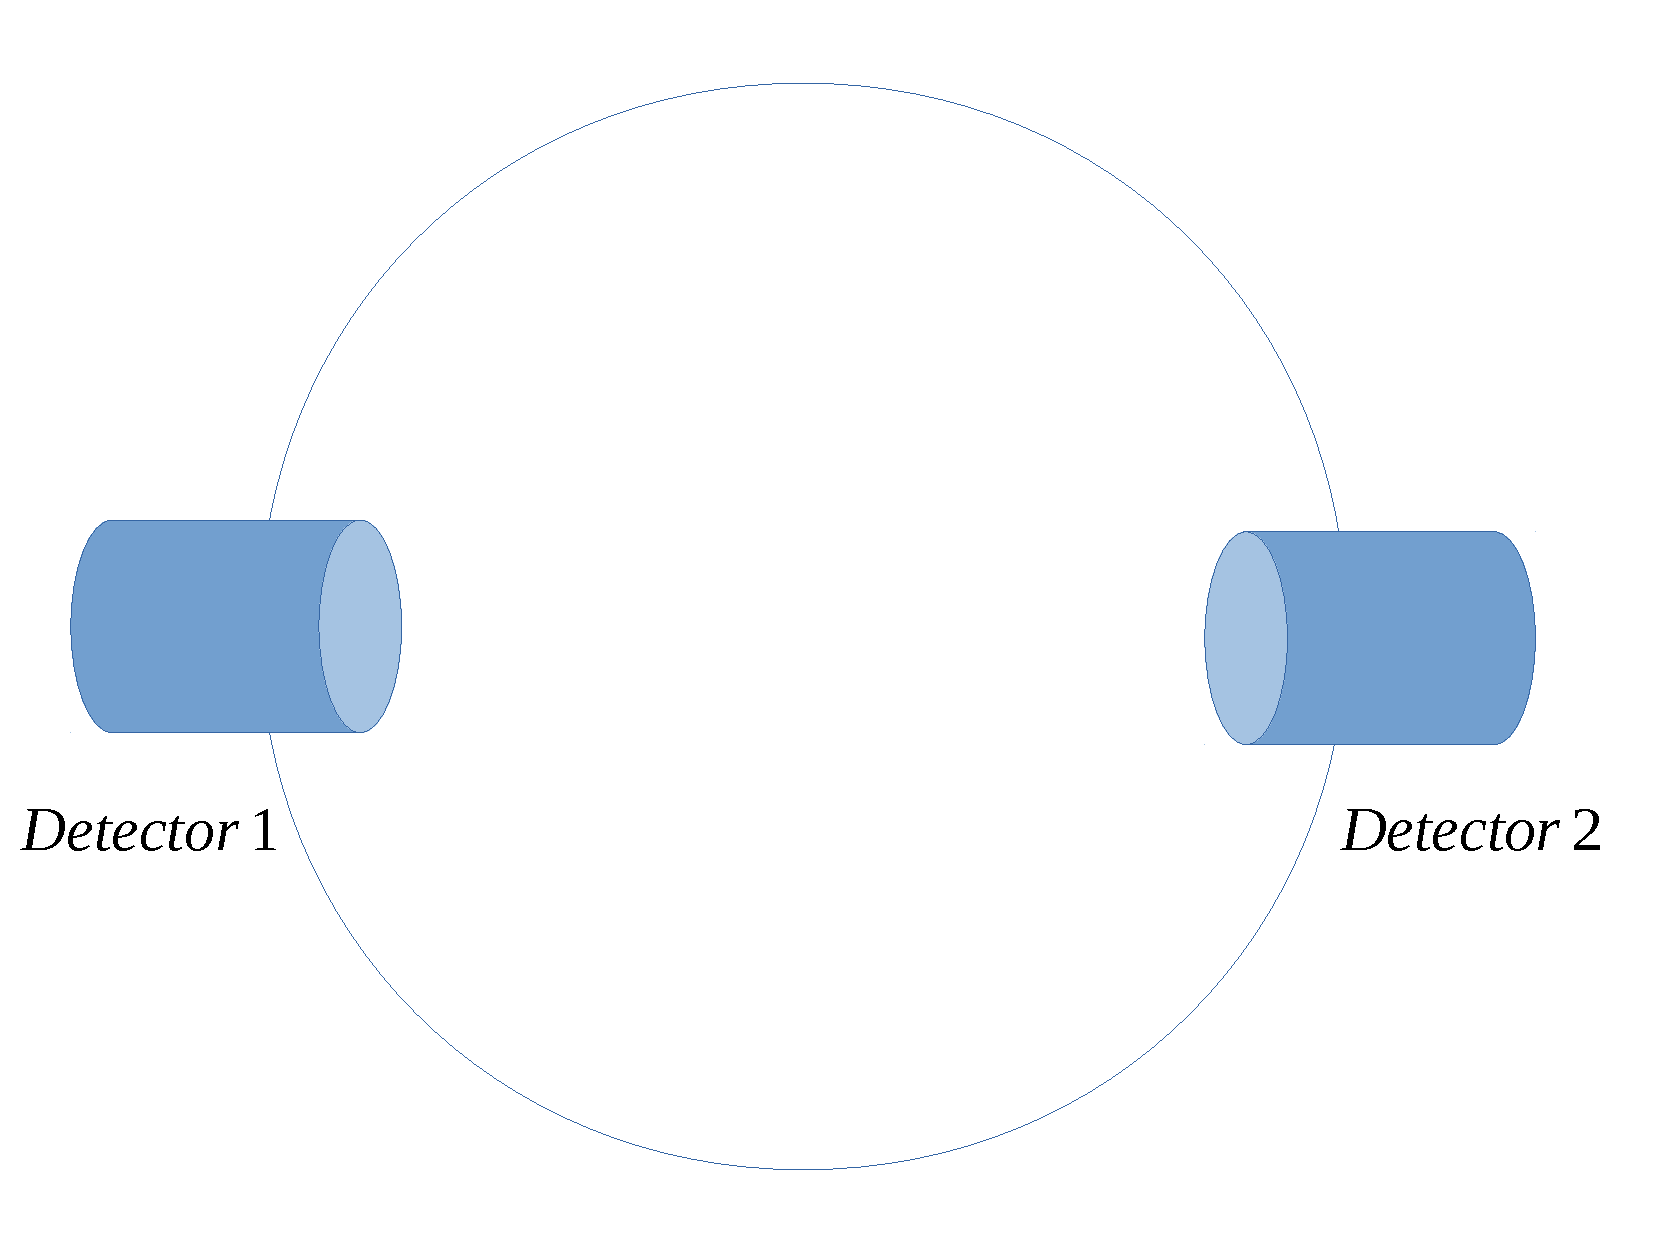
\includegraphics[width = 0.5\textwidth]{conf_two}
\caption{Experimental setup for two $\gamma$ decay.}
\label{Fig: exp setup for 2gamma}
\end{figure}

\begin{figure}[H]
\centering
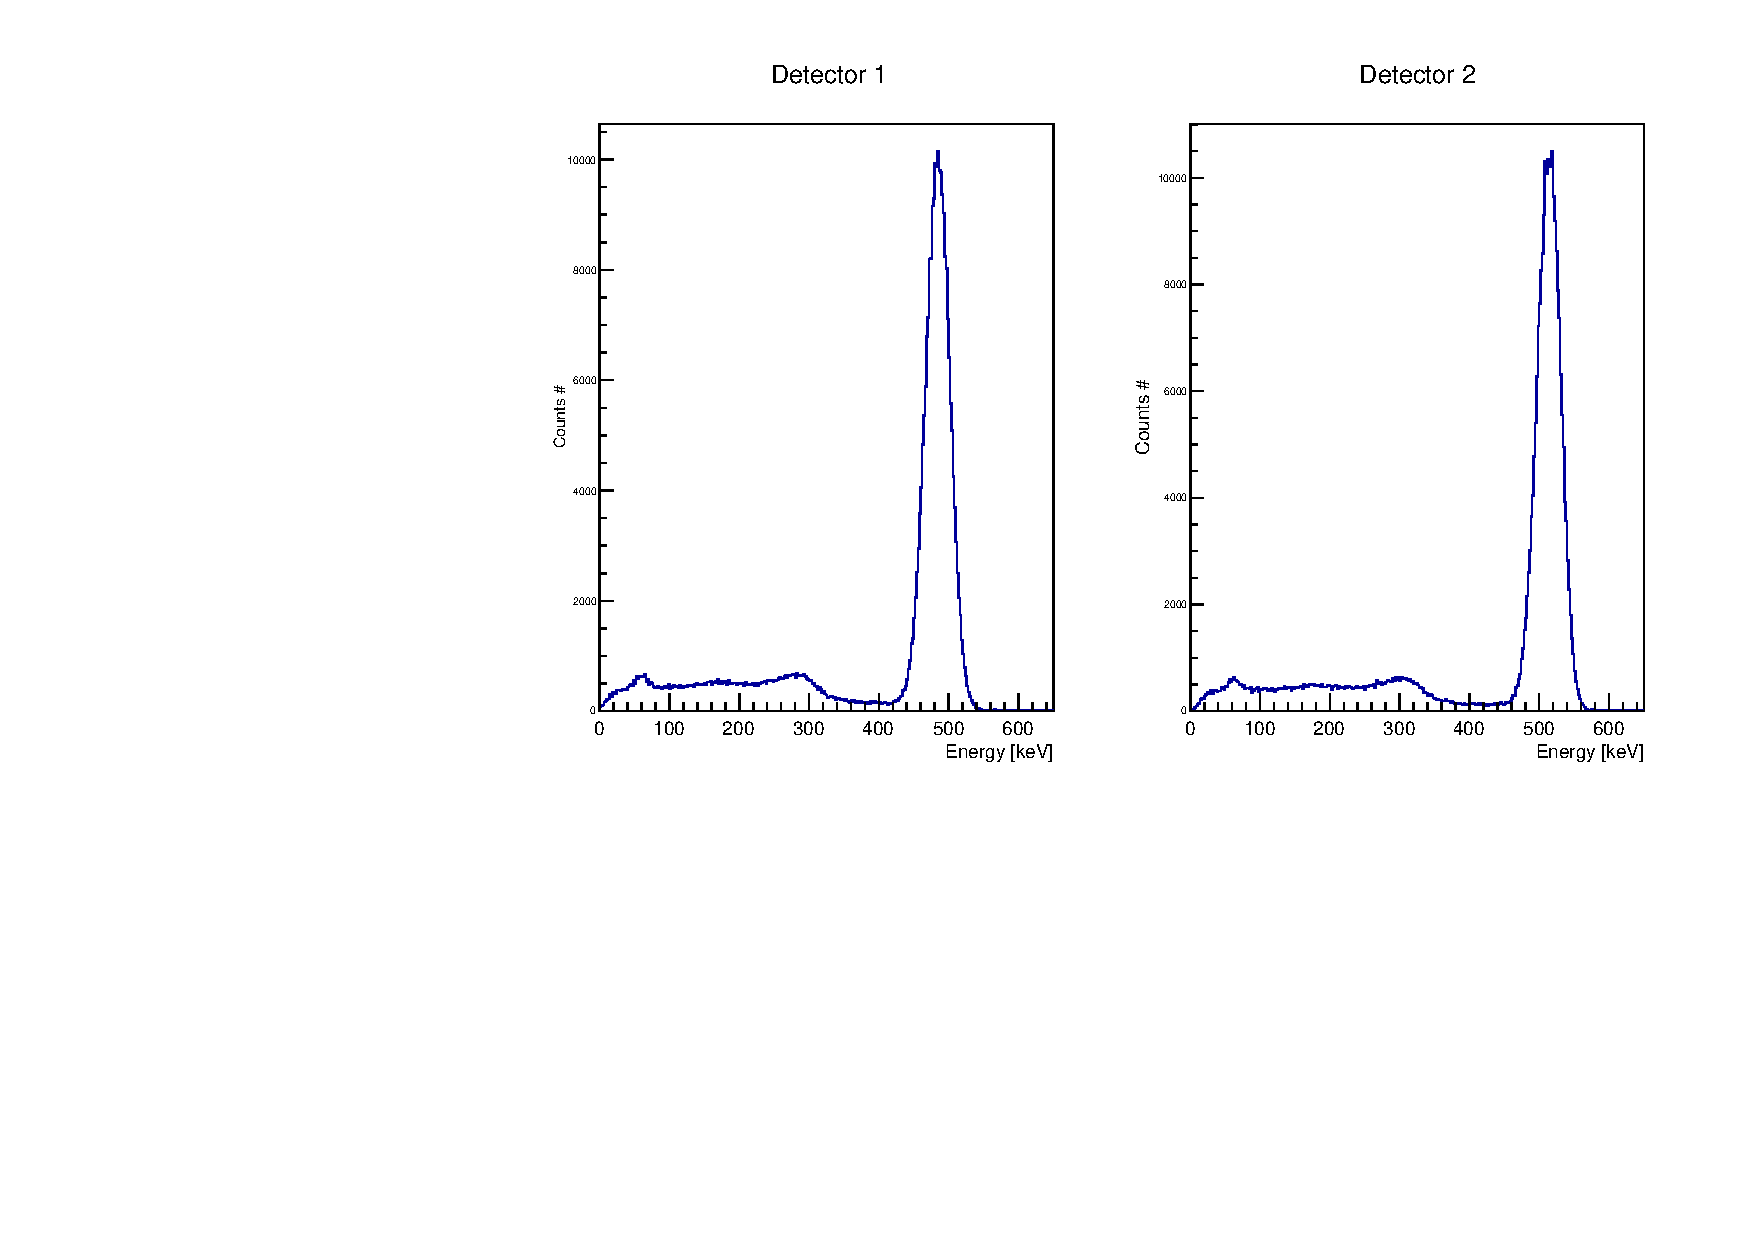
\includegraphics[width = 0.8\textwidth]{two_coinc_wbg}
\caption{2-$\gamma$ coincidence. From configuration 1}
\label{Fig: 2gamma coinc with bg}
\end{figure}

In order to determine the number of detected para-positronium decay events, the photopeak has to be integrated.
Before integrating the photopeak, however, the Compton Background has to be removed as in Fig \ref{Fig: removed compton back}.

\begin{figure}[H]
\centering
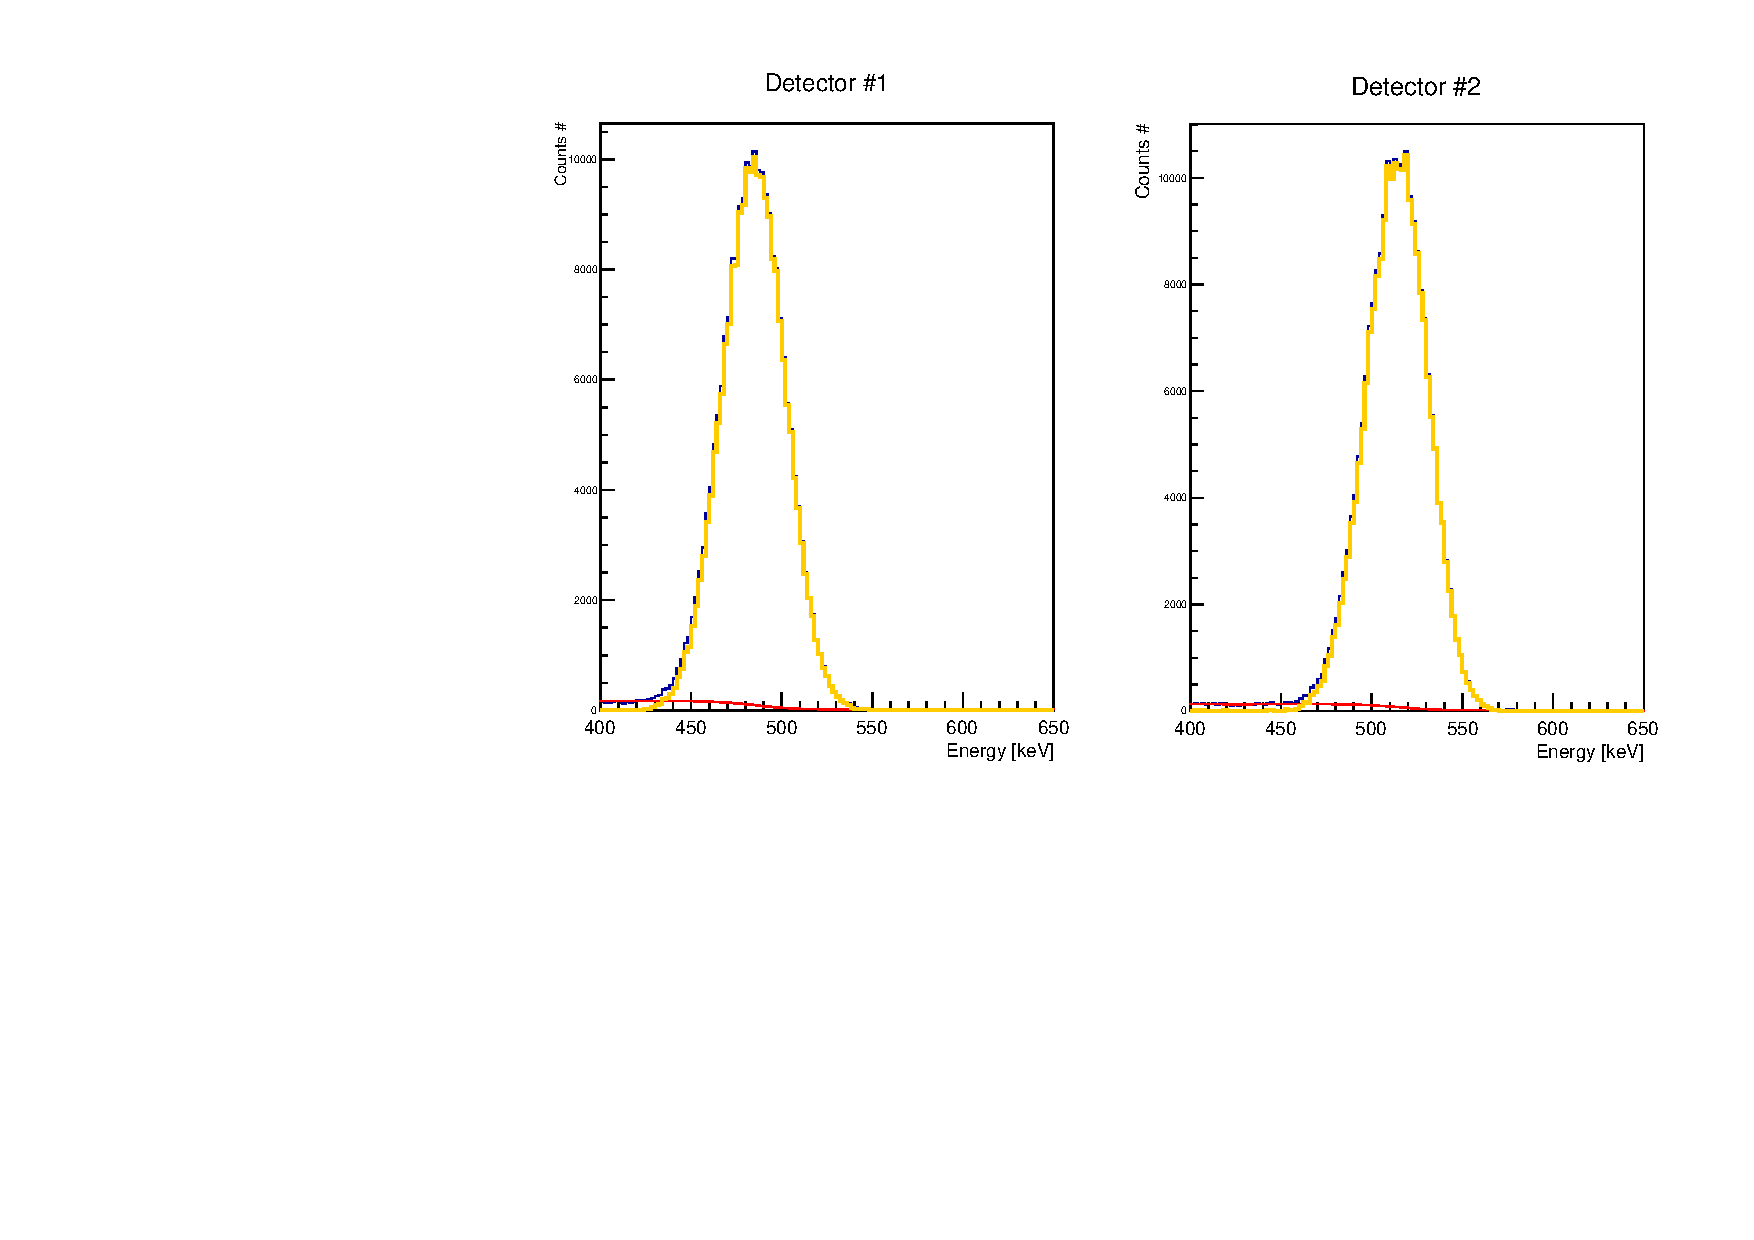
\includegraphics[width = 0.8\textwidth]{coinc_back}
\caption{2-$\gamma$ coincidence with removed background.}
\label{Fig: removed compton back}
\end{figure}

After that the photopeak could be integrated resulting in a yields of:
\begin{equation}
N_{2\gamma} = 218248
\end{equation} 

The number of obtained events has to be corrected due to the fact that not all para positronium decay events are detected and then counted. With the purpose of correcting this measure, we need an estimate of the covered solid angle in this configuration:
\begin{equation}
f_{2\gamma} = \dfrac{2\pi r^2}{4\pi d}
\end{equation}
that lead to an estimate for the number of parapositronium decay events of:
\begin{equation}
N_{2\gamma} = \dfrac{N_{2\gamma}^{\text{measured}}}{f_{2\gamma}}
\end{equation}




